\documentclass{beamer}

\usepackage{amssymb,amsmath}
\usepackage{xcolor}
\usepackage{cancel}
\usepackage{array}



%\mode<draft>
\mode<presentation>
{
  \usetheme{Goettingen}
  \setbeamercovered{transparent=20}
  \usecolortheme{crane}
}


\usepackage[english]{babel}
\usepackage[latin1]{inputenc}
\usepackage{times}
%\usepackage[T1]{fontenc}
% Or whatever. Note that the encoding and the font should match. If T1
% does not look nice, try deleting the line with the fontenc.



%%%%%% MY COMMANDS %%%%%%

%%% Rate variables:
\newcommand{\crossSec} {{\sigma_\mathrm{prod}}}
\newcommand{\Lu}             {{\cal L}}  % Luminosity
\newcommand{\Br}              {{\cal B}}  % Branching ratio



%%% Units:
\newcommand{\tev}   {{\rm TeV}}
\newcommand{\gev}   {{\rm GeV}}
\newcommand{\invfb} {{\rm fb}^{-1}}



%%% mSUGRA:
\newcommand{\mzero} {m_{0}}
\newcommand{\mhalf} {m_{1/2}}
\newcommand{\azero} {A_{0}}
\newcommand{\tanb}  {\tan\beta}



%%% SUSY particles:
\newcommand{\gluino}          {\tilde{g}}
\newcommand{\squark}[1]       {\tilde{q}_{#1}}
\newcommand{\squarkup}[1]     {\tilde{u}_{#1}}
\newcommand{\squarkdown}[1]   {\tilde{d}_{#1}}
\newcommand{\squarktop}[1]    {\tilde{t}_{#1}}
\newcommand{\squarkbottom}[1] {\tilde{b}_{#1}}
\newcommand{\staupm}[1]       {\tilde{\tau}_{#1}^{\pm}}
\newcommand{\stau}[1]         {\tilde{\tau}_{#1}}
\newcommand{\smu}[1]          {\tilde{\mu}_{#1}}
\newcommand{\sel}[1]          {\tilde{e}_{#1}}
\newcommand{\slepton}[1]      {\tilde{\ell}_{#1}}
\newcommand{\schizero }[1]    {\tilde{\chi}_{#1}^{0}}
\newcommand{\schipm }[1]      {\tilde{\chi}_{#1}^{\pm}}



%%% Event variables:
\newcommand{\met}        {{E\!\!\!\!/_{\rm T}}}
\newcommand{\etof}[1]    {E_{{\rm T}, #1}}
\newcommand{\ptof}[1]    {p_{{\rm T}, #1}}
\newcommand{\ptvisof}[1] {p_{{\rm T}, #1}^{\rm vis}}
\newcommand{\et}         {E_{\rm T}}
\newcommand{\pt}         {p_{\rm T}}
\newcommand{\ptvis}      {p_{\rm T}^{\rm vis}}



%%% Kinematic Observables:
\newcommand{\mtautau}[1] {m_{\tau\tau}^{#1}}
\newcommand{\mtaumu}[1] {m_{\tau\mu}^{#1}}
\newcommand{\ptslope}{{\rm slope}(\ptvisof{\tau})}
\newcommand{\ptslopeHigh}{{\rm slope}(\ptvisof{\tau ({\rm high}) })}
\newcommand{\ptslopeLow}{{\rm slope}(\ptvisof{\tau ({\rm low}) })}
\newcommand{\ptslopePlus}{{\rm slope}(p_{\rm T\ +}^{\rm vis}) }
\newcommand{\ptslopeMean} {\left<\ptslope\right>}



%%% MC tools:
\newcommand{ \superbayes} {{\tt SuperBayeS}}
\newcommand{ \fittino} {{\tt Fittino}}
\newcommand{ \mastercode} {{\tt MasterCode}}
\newcommand{ \gambit} {{\tt \color{red} GAMBIT}}
\newcommand{ \prospino } {{\tt PROSPINO}}
\newcommand{ \vbfnlo } {{\tt VBFNLO}}
\newcommand{ \spheno } {{\tt SPheno}}
\newcommand{ \madgraph } {{\tt MadGraph 5}}
\newcommand{ \pythia } {{\tt PYTHIA 8}}
\newcommand{ \isajet } {{\tt ISAJET}}
\newcommand{ \delphes } {{\tt Delphes 3}}
\newcommand{ \pgs }    {{\tt PGS4}}



%%% Special variables:
\newcommand{\Li}[2] {{\cal L}^{#2}_{#1}}  % Likelihood
\newcommand{\Lirm}[2] {{\cal L}^\mathrm{#2}_\mathrm{#1}}  % Likelihood
\newcommand{\deltaLFV} {\delta_{RR, {\rm LFV}} }
\newcommand{\tauh} {\tau_{\rm h} }
\newcommand{\emm} {\mathcal{M} }



%%% Custom colors:
\definecolor{brick}{rgb}{0.9, 0.3, 0}
\definecolor{sand}{rgb}{1, 0.6, 0}
\definecolor{hidebrick}{rgb}{0.99, 0.8, 0.5}
\definecolor{hidesand}{rgb}{1., 0.7, 0.7}
\definecolor{smoke}{gray}{0.15}
\definecolor{algae}{rgb}{0, 0.85, 0.65}
\definecolor{seafoam}{rgb}{0.3, 1, 0.95}
\setbeamercolor{seabox}{fg=black,bg=seafoam}



%%% Customized beamer templates:
\newenvironment<>{negativeblock}[1]{%
  \begin{actionenv}#2%
    \def\insertblocktitle{#1}%
      \par%
      \mode<presentation>{%
        \setbeamercolor{block title}{fg=black,bg=brick}
        \setbeamercolor{block body}{fg=smoke,bg=sand}
        \setbeamercolor{block title example}{fg=normal,bg=hidebrick}
        \setbeamercolor{block body example}{fg=normal,bg=hidesand}
        \setbeamercolor{itemize item}{fg=smoke}
        \setbeamertemplate{itemize item}{$\neg$}
      }%
      \usebeamertemplate{block begin}}
    {\par\usebeamertemplate{block end}\end{actionenv}}
    
\newenvironment<>{positiveblock}[1]{%
  \begin{actionenv}#2%
    \def\insertblocktitle{#1}%
      \par%
      \mode<presentation>{%
        \setbeamercolor{block title}{fg=black,bg=algae}
        \setbeamercolor{block body}{fg=smoke,bg=seafoam}
        \setbeamercolor{itemize item}{fg=smoke}
        \setbeamertemplate{itemize item}[square]
      }%
      \usebeamertemplate{block begin}}
    {\par\usebeamertemplate{block end}\end{actionenv}}
    
\addtobeamertemplate{title page}{}{\vspace{1cm} \centering
    
\includegraphics[height=1cm]{OKlogo_blue.jpg}~
\includegraphics[height=1cm]{logo_su_en_big_dark_blue.jpg}}
%%%%%%





\title[Next Gen Global Fits with LHC \hspace{1cm} \insertframenumber/\inserttotalframenumber]
{Towards Next Generation Global Fits Including LHC Simulations}

\logo{
\includegraphics[width=1.5cm]{Logo_Final.png}}

\author[Abram Krislock\\ Oct 22\\ Partikeldagarna 2013\\ \insertlogo]
{Abram Krislock}

\institute[OKC, SU]
{Oskar Klein Centre, Stockholm University}

\date[Partikeldagarna 2013]
{Partikeldagarna 2013}

\AtBeginSection[]
{
  \begin{frame}<beamer>
    \frametitle{Outline}
    \tableofcontents[currentsection]
  \end{frame}
}

\begin{document}

\begin{frame}
  \titlepage
\end{frame}

\begin{frame}
  \frametitle{Outline}
  \tableofcontents
\end{frame}



\section{Motivation}
\subsection{... Why global fits?}

\begin{frame}
  \frametitle{... Why global fits?}
  \begin{block}{Standard Model \emph{must} be incomplete}
    \begin{tabular}{cc}
      \visible<2->{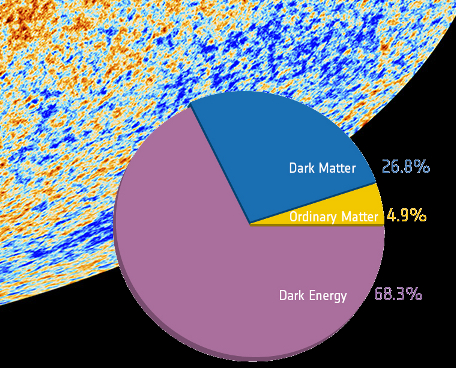
\includegraphics[width=4cm]{dark-pie.jpg}} &
      \visible<3->{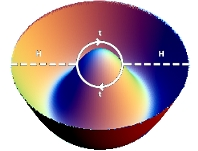
\includegraphics[width=4cm]{Higgs-mass-divergence.jpg}} \\
      \visible<4->{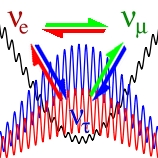
\includegraphics[width=3cm]{neutrino-oscillation.jpg}} &
      \visible<5->{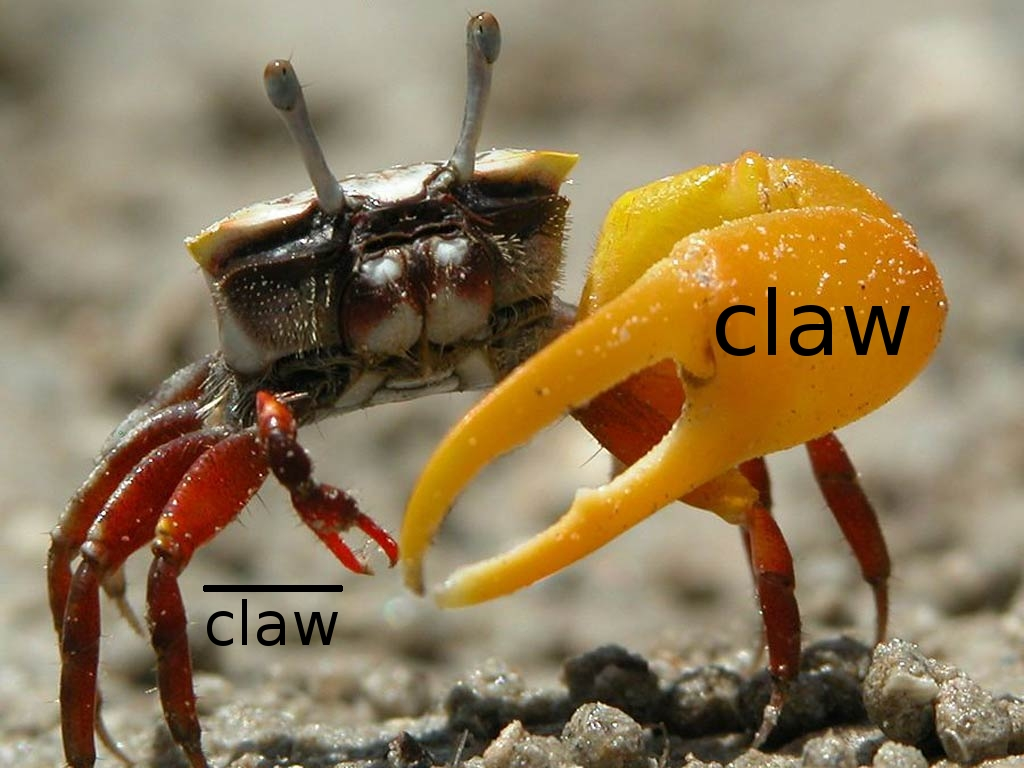
\includegraphics[width=4cm]{asymmetry.jpg}}
    \end{tabular}
  \end{block}
\end{frame} 

\begin{frame}
  \frametitle{Beyond the Standard Model}
  {\huge$\left[\mathrm{ERROR:\ BSM\ not\ found!!}\right]$} \\ \vspace{0.5cm}
  Many experiments have set many limits on various BSM scenarios. \\ \vspace{1cm}
  \pause ``Considering those limits, how does my model fare? Is it ruled out?''
\end{frame} 

\begin{frame}
  \frametitle{Global Fits and Statistical Inferencing}
  \begin{block}{Simple BSMs with very few parameters}
    \begin{itemize}
      \item Overlap limits from different experimental searches
      \item Statistically combine limits: Composite Likelihood
      \item See ``surviving parameter space''
    \end{itemize}
  \end{block}
  \vspace{-0.3cm} \pause
  \begin{positiveblock}{Complicated BSMs with many parameters}
    Absolutely need \emph{Global Fits}!!
    \begin{itemize}
      \item Smart scanning algorithms to scan huge parameter spaces!!
      \item Proper treatment of input uncertainties: Nuisance parameters!!
      \item Interpretation: Bayesian / Frequentist??
      \item Projection to interesting parameter planes.
    \end{itemize}
  \end{positiveblock}
\end{frame} 



\section{A New Global Fit Framework}
\subsection{... Why have a new one??}

\begin{frame}
  \frametitle{... Why have a new global fit framework??}
  Existing global fit frameworks have shortcomings:
  \begin{negativeblock}{\superbayes, \fittino, \mastercode, ...}
    \begin{itemize}
      \item Restricted to either Bayesian or Frequentist interpretations
      \pause \item Restricted to a particular model (SUSY)
      \pause \item Restricted to a particular set of theory tools
      \pause \item Sub-optimal scanning algorithms
      \pause \item Only direct use or simple extrapolation of LHC and Astrophysics limits
      \pause \item Sometimes a black box... Codes are not made public
    \end{itemize}
  \end{negativeblock}
  \pause Thus, we have started work on \gambit.
\end{frame} 



\subsection{... Okay, so what's GAMBIT?}

\begin{frame}
  \frametitle{... Okay, so what's \gambit?}
  \vspace{-0.2cm}
  \begin{block}{{\color{red}G}lobal {\color{red}A}nd {\color{red}M}odular {\color{red}B}SM {\color{red}I}nference {\color{red}T}ool}
    Design principles of \gambit: Flexibility and Modularity
      \begin{itemize}
        \pause\item Entire \gambit\ framework designed to be as easy as possible to add additional
        \begin{itemize}
          \item Models
          \item Experimental data sets and limits
          \item Scanning algorithms
        \end{itemize}
        \pause\item Frequentist or Bayesian methods with customizable
        \begin{itemize}
          \item Likelihoods
          \item Priors
          \item Nuisance parameters
        \end{itemize}
        \pause\item Intuitive interface connecting \gambit\ with external physics tools
        \item Plug'n'play swapping of physics tools, scanners, and likelihoods
        \item Open source release
    \end{itemize}
    \pause \begin{beamercolorbox}{seabox}
          {\small $\Lirm{GAMBIT}{} = \Lirm{Direct}{DM} \times \Lirm{Indirect}{DM} 
          \times \Li{\mathrm{Relic}\Omega}{\mathrm{DM}} \times \Lirm{LHC}{} \times \Lirm{Flavor}{} \times \Lirm{Higgs}{} \cdots$}
    \end{beamercolorbox}
  \end{block}
\end{frame} 



\subsection{... Who is working on GAMBIT?}

\begin{frame}
  \frametitle{... Who is working on \gambit?}
  22 Members from 13 Institutes:
  \begin{positiveblock}{The \gambit\ Collaboration}
    \centering
    C.~Bal\'{a}zs, T.~Bringmann, A.~Buckley, J.~Conrad, J.~Cornell, L.~A.~Dal, J.~Edsj\"{o}, B.~Farmer, P.~Jackson, A.~Krislock, A.~Kvellestad, F.~N.~Mahmoudi, G.~Martinez, A.~Putze, A.~Raklev, C.~Rogan, A.~Saavedra C.~Savage, P.~Scott, N.~Serra, C.~Weniger, M.~White
  \end{positiveblock}
  8 Experiments: \\ \hspace{0.5cm}
  \begin{beamercolorbox}{seabox}
    \centering
    Fermi-LAT, IceCube, ATLAS, LHCb,\\ HESS, AMS-02, CTA, DARWIN
  \end{beamercolorbox}
\end{frame}



\section{LHC Simulation within a Global Fit}
\subsection{... Why not just use the limits?}

\begin{frame}
  \frametitle{... Why not just use the limits?}
  \begin{block}{ATLAS and CMS SUSY searches}
    \begin{itemize}
      \item CMSSM / mSUGRA limits
      \item Simplified Model limits
    \end{itemize}
  \end{block}
  \begin{negativeblock}{Can the limits really apply...? Generally not!!}
    \begin{itemize}
      \pause \item nuSUGRA, other $\cancel{\mathrm{SUSY}}$ schemes
      \pause \item PMSSM
      \pause \item BSM, not SUSY, but SUSY-like signals
    \end{itemize}  
  \end{negativeblock}
\end{frame} 

\begin{frame}
  \frametitle{Simulation Required}
  To perform a global fit of a particular model...
  \begin{positiveblock}{Monte Carlo LHC Simulation Chain}
    \scriptsize \begin{tabular}{c|ccc}
      \visible<2->{$\{\crossSec,~\Br\}_\mathrm{processes}$} & 
              \visible<3->{\begin{tabular}{c} \prospino \\ \vbfnlo \\ \emph{etc.} \\ $\searrow$ \end{tabular}} & &
              \visible<3->{\begin{tabular}{c} \spheno \\ \madgraph \\ \emph{etc.} \\ $\swarrow$ \end{tabular}} \\
      \visible<4->{$\downarrow$} \\
      \visible<4->{\begin{tabular}{c} Collision Events \\ Parton Showering \\ ISR \& FSR \end{tabular}} & &
              \visible<5->{\begin{tabular}{c} \pythia \\ \isajet \\ \emph{etc.} \\ $\downarrow$ \end{tabular}} \\
      \visible<6->{$\downarrow$} & & & \\
      \visible<6->{\begin{tabular}{c} Detector Sim \\ Perform Analyses \end{tabular}} & &
              \visible<7->{\begin{tabular}{c} \delphes \\ \pgs \\ \emph{etc.} \\ $\downarrow$ \\ \{Analyses\} \end{tabular}}
    \end{tabular}
  \end{positiveblock}
  ... For each and every point within your likelihood scan.
\end{frame} 



\subsection{... Are you nuts?!}

\begin{frame}
  \frametitle{... Are you nuts?!}
  {\Huge Yes.}
  \begin{tabular} {cc}
      \visible<2->{
\includegraphics[width = 4cm]{what-nuts.jpg}} &
      \visible<3->{
\includegraphics[width = 4cm]{youre-both-nuts.jpg}}
  \end{tabular}
\end{frame} 

\begin{frame}
  \frametitle{... But not so nuts: Speed Tricks}
  \begin{block}{How to get more speed?}
    \begin{tabular}{l}
      \visible<2->{\color{red} $\blacktriangleright$ Speed up $\crossSec$ calculation} \\
      \visible<3->{\color{blue} $\blacktriangleright$ Parallelization with production processes in mind} \\
      \visible<4->{\color{brown} $\blacktriangleright$ Turn off parts of Monte Carlo, then tune analyses}
    \end{tabular}
  \end{block}
  \begin{positiveblock}{Monte Carlo LHC Simulation Chain}
    {\scriptsize \begin{tabular}{ccc}
      \begin{tabular}{cc} \visible<2->{\color{red} \begin{tabular}{c} LO $\crossSec$ \\ conservative \end{tabular} } &
                  \visible<2->{\color{red} $\Leftarrow$} \end{tabular} &
              \only<1>{$\{\crossSec,~\Br\}_\mathrm{processes}$}\only<2>{$\{{\color{red}\crossSec},~\Br\}_\mathrm{processes}$}\only<3->{$\{{\color{red}\crossSec},~\Br\}_\mathrm{\color{blue}\bf processes}$} &
              \begin{tabular}{cc} \visible<2->{\color{red} $\Rightarrow$} &
                  \visible<2->{\color{red} \begin{tabular}{c} Neural Network \\ Fast NLO $\crossSec$ \end{tabular} }
              \end{tabular}  \\
      \visible<3->{\color{blue} $\swarrow$} & \only<1-2>{$\downarrow$}\only<3->{\color{blue}$\downarrow$} &
              \visible<3->{\color{blue} $\searrow$} \\
      \visible<3->{\tiny\color{blue}\bf \begin{tabular}{c} Parallelized \\ Collision Events \\
                      \only<1-3>{Parton Showering}\only<4->{\color{brown}\cancel{Parton Showering}} \\
                      \only<1-3>{ISR \& FSR}\only<4->{\color{brown}\cancel{ISR \& FSR}}
                      \end{tabular} } &
              \only<1-2>{\tiny \begin{tabular}{c} Parallelized \\ Collision Events \\
                      \only<1-3>{Parton Showering}\only<4->{\color{brown}\cancel{Parton Showering}} \\
                      \only<1-3>{ISR \& FSR}\only<4->{\color{brown}\cancel{ISR \& FSR}}
                      \end{tabular} }\only<3->{\tiny\color{blue}\bf \begin{tabular}{c} Parallelized \\ Collision Events \\
                      \only<1-3>{Parton Showering}\only<4->{\color{brown}\cancel{Parton Showering}} \\
                      \only<1-3>{ISR \& FSR}\only<4->{\color{brown}\cancel{ISR \& FSR}}
                      \end{tabular} } &
              \visible<3->{\tiny\color{blue}\bf \begin{tabular}{c} Parallelized \\ Collision Events \\
                      \only<1-3>{Parton Showering}\only<4->{\color{brown}\cancel{Parton Showering}} \\
                      \only<1-3>{ISR \& FSR}\only<4->{\color{brown}\cancel{ISR \& FSR}}
                      \end{tabular} } \\
      \visible<3->{\color{blue} $\downarrow$} & \only<1-2>{$\downarrow$}\only<3->{\color{blue}$\downarrow$} & 
              \visible<3->{\color{blue} $\downarrow$} \\
      \visible<3->{\tiny\color{blue}\bf \begin{tabular}{c}
                      \only<1-3>{Detector Sim}\only<4->{\color{brown}\cancel{Detector Sim}} \\
                      Perform \only<1-3>{Analyses}\only<4->{\color{brown}Analyses}
                      \end{tabular} } &
              \only<1-2>{\tiny \begin{tabular}{c}
                      \only<1-3>{Detector Sim}\only<4->{\color{brown}\cancel{Detector Sim}} \\
                      Perform \only<1-3>{Analyses}\only<4->{\color{brown}Analyses}
                      \end{tabular} }\only<3->{\tiny\color{blue}\bf \begin{tabular}{c}
                      \only<1-3>{Detector Sim}\only<4->{\color{brown}\cancel{Detector Sim}} \\
                      Perform \only<1-3>{Analyses}\only<4->{\color{brown}Analyses}
                      \end{tabular} } &
              \visible<3->{\tiny\color{blue}\bf \begin{tabular}{c}
                      \only<1-3>{Detector Sim}\only<4->{\color{brown}\cancel{Detector Sim}} \\
                      Perform \only<1-3>{Analyses}\only<4->{\color{brown}Analyses}
                      \end{tabular} }
    \end{tabular} }
  \end{positiveblock}
  \visible<5>{Each trick reduces time for $\Lirm{LHC}{}$.}
\end{frame} 



\section*{Summary}

\begin{frame}
  \frametitle{Summary}
  \begin{columns}
    \column[c]{0.6\textwidth}
    \begin{itemize}
      \item \gambit\ is coming!
      \item Flexibility \& Modularity
      \item Open Source \& Customizability
      \item Smart \& Fast LHC Simulations
      \begin{itemize}
        \item Speedy $\crossSec$ calculations
        \item Process dependent parallelization
        \item Simplified Monte Carlo
      \end{itemize}
    \end{itemize}
    \column[c]{0.4\textwidth}
    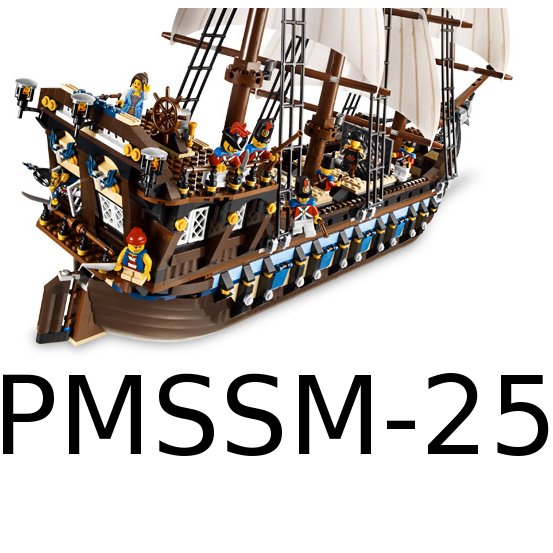
\includegraphics[width=4cm]{flagship.jpg}
  \end{columns}
\end{frame}

\end{document}


